\documentclass[tikz, preview]{standalone}

\usepackage{amsfonts, amsthm, amssymb, amsmath, stmaryrd, etoolbox}
\usepackage{tikz}
\usepackage[all,2cell]{xy}
\usetikzlibrary{matrix,arrows,shapes,decorations.markings,decorations.pathreplacing}
\definecolor{rewritecolor}{rgb}{0,.9,1}
\tikzset{rewritenode/.style={shape=circle,fill=rewritecolor,scale=0.25,font=\Huge}}
\tikzset{RWopen/.style={shape=circle,draw=black,fill=white,scale=0.5,font=\Huge}}
\tikzset{RWclosed/.style={shape=circle,fill=black,scale=0.5,font=\Huge}}
\tikzset{CDnode/.style={shape=circle,fill=white,scale=.5}}
\tikzset{zxgreen/.style={shape=circle,draw,thick,fill=green}}
\tikzset{zxred/.style={shape=circle,draw,thick,fill=red}}
\tikzset{zxyellow/.style={shape=rectangle,draw,thick,fill=yellow}}
\tikzset{zxdiamond/.style={shape=diamond,fill=black,inner sep=2.75}}
\tikzset{zxopen/.style={shape=circle,draw,thick,inner sep=2pt}}
\tikzset{->-/.style={decoration={markings,mark=at position .5 with {\arrow{>}}},postaction={decorate}}}

\begin{document}
\[
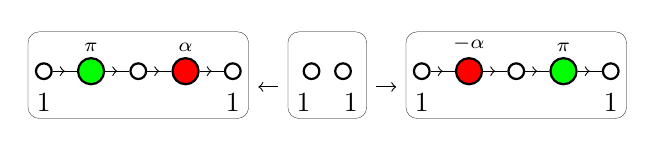
\begin{tikzpicture}
%
%
%
\begin{scope}[shift={(-0.5,-0.6)}]
\node [zxopen] (v1) at (-1.1,0.2) {};
\node [zxgreen,label={[shift={(0,-0.05)}]\scriptsize $\pi$}] (v2) at (-0.5,0.2) {};
\node [zxred,label={[shift={(0,-0.05)}]\scriptsize $\alpha$}] (v3) at (0.7,0.2) {};
\node [zxopen] (v4) at (1.3,0.2) {};	
\node [zxopen] (v8) at (0.1,0.2) {};
%
\draw [->-] (v1) to (v2);
\draw [->-] (v2) to (v8);
\draw [->-] (v8) to (v3);
\draw [->-] (v3) to (v4);
%
\node at (-1.1,-0.2) {$1$};
\node at (1.3,-0.2) {$1$};
\node (v11) at (1.5,0) {};
\draw [ultra thin, rounded corners] (-1.3,0.7) rectangle (1.5,-0.4);
\end{scope}
%
%
%
\begin{scope}[shift={(3.1,-0.1)}]
\node [zxopen] (v1) at (-1.3,-0.3) {};
\node [zxopen] (v3) at (-0.9,-0.3) {};
%
\draw [ultra thin, rounded corners] (-1.6,0.2) rectangle (-0.6,-0.9);
\node at (-1.4,-0.7) {$1$};
\node at (-0.8,-0.7) {$1$};
\node (v12) at (-1.6,-0.5) {};
\node (v14) at (-0.6,-0.5) {};
\end{scope}
%
%
%
\begin{scope}[shift={(4.3,-0.6)}]
\node [zxopen] (v1) at (-1.1,0.2) {};
\node [zxred,label={[shift={(0,-0.05)}]\scriptsize $-\alpha$}] (v2) at (-0.5,0.2) {};
\node [zxgreen,label={[shift={(0,-0.05)}]\scriptsize $\pi$}] (v3) at (0.7,0.2) {};
\node [zxopen] (v4) at (1.3,0.2) {};
\node [zxopen] (v8) at (0.1,0.2) {};
%
\draw [->-] (v1) to (v2);
\draw [->-] (v2) to (v8);
\draw [->-] (v8) to (v3);
\draw [->-] (v3) to (v4);
%
\node at (-1.1,-0.2) {$1$};
\node at (1.3,-0.2) {$1$};
\node (v15) at (-1.3,0) {};
\draw [ultra thin, rounded corners] (-1.3,0.7) rectangle (1.5,-0.4);
\end{scope}
%
%
%
\draw [<-] (v11) edge (v12);
\draw [->] (v14) edge (v15);
\end{tikzpicture}
\]
\end{document}
